\section{Fast problem analysis}

First, we have to resolve the main problem that comes from the requirement analysis: we said that the robot has a controller board such as \texttt{Arduino} or \texttt{Raspberry} and that it must communicate with \texttt{Android}. 

Notice that even if the robot is a \texttt{mBot}, we can easily mount a \texttt{Raspberry} over \texttt{Arduino}, so we can use all the framework and the technologies that works with \texttt{Linux}.
Then \textbf{we consider that the robot is controlled by a \texttt{Raspberry} that is well configured}.

\begin{tcolorbox}
	\begin{center}
		\textbf{Since we have the \texttt{BasicRobot} already developed and working, we decide to use it in order to build a very simple demo of the system with a \texttt{mBot} with a \texttt{Raspberry} installed over \texttt{Arduino}.}
	\end{center}
\end{tcolorbox}

\subsection{Connection between \texttt{Android} and \texttt{Arduino}}

As shown in the fast requirement analysis, from the \texttt{Android} point of view we have large set of instruments to develop using Bluetooth or Wi-Fi Direct, but we can't say the same thing from the \texttt{Raspberry} (Linux) point of view.

\begin{tcolorbox}
	\begin{center}
		\textbf{We choose to use Bluetooth for communication because we have found \textit{poor} support for \texttt{Wi-Fi Direct} and also because we think that Bluetooth can consume less.}
	\end{center}
\end{tcolorbox}

Even if there are a working \texttt{Python} implementation of Bluetooth for Linux, we decided to make a fast porting of it because the \texttt{QAK} is written in \texttt{Kotlin}.

The entire ported library, called \textcolor{ForestGreen}{\texttt{KBluez}} is fully accessible at this \texttt{GitHub} \href{https://github.com/LM-96/MobileSystemProject/tree/main/kBluez}{repository}.
Basically, there is a \texttt{Python} script (\href{https://github.com/LM-96/MobileSystemProject/blob/main/kBluez/lib/src/main/resources/python/pybluezwrapper.py}{\textcolor{MidnightBlue}{\texttt{pybluezwrapper.py}}}) launched by the \texttt{Kotlin} library as a system process using \href{https://docs.oracle.com/en/java/javase/18/docs/api/java.base/java/lang/Runtime.html}{\texttt{Java Runtime}}: \texttt{stdin}, \texttt{stdout} and \texttt{stderr} of the \texttt{Python} script are captured and handled by \texttt{Kotlin} that is able to send commands to \texttt{PyBluez} and read response by using a proper protocol.

Indeed, \texttt{pybluezwrapper.py} uses the main thread for reading commands from \texttt{stdin} that are sent by \texttt{Kotlin} as \href{https://en.wikipedia.org/wiki/JSON}{json} strings. When the \texttt{Python} script receives the command to open a \textit{Bluetooth Socket}, so \texttt{pybluezwrapper.py} launches another thread and entrust the new socket to it associating an unique identifier that \texttt{Kotlin} uses to refer to. \textbf{In this way, concurrency is safely guaranteed}, and it's possible to open multiple sockets without blocking the \texttt{Python} script.

\begin{figure}[h!]
	\centering
	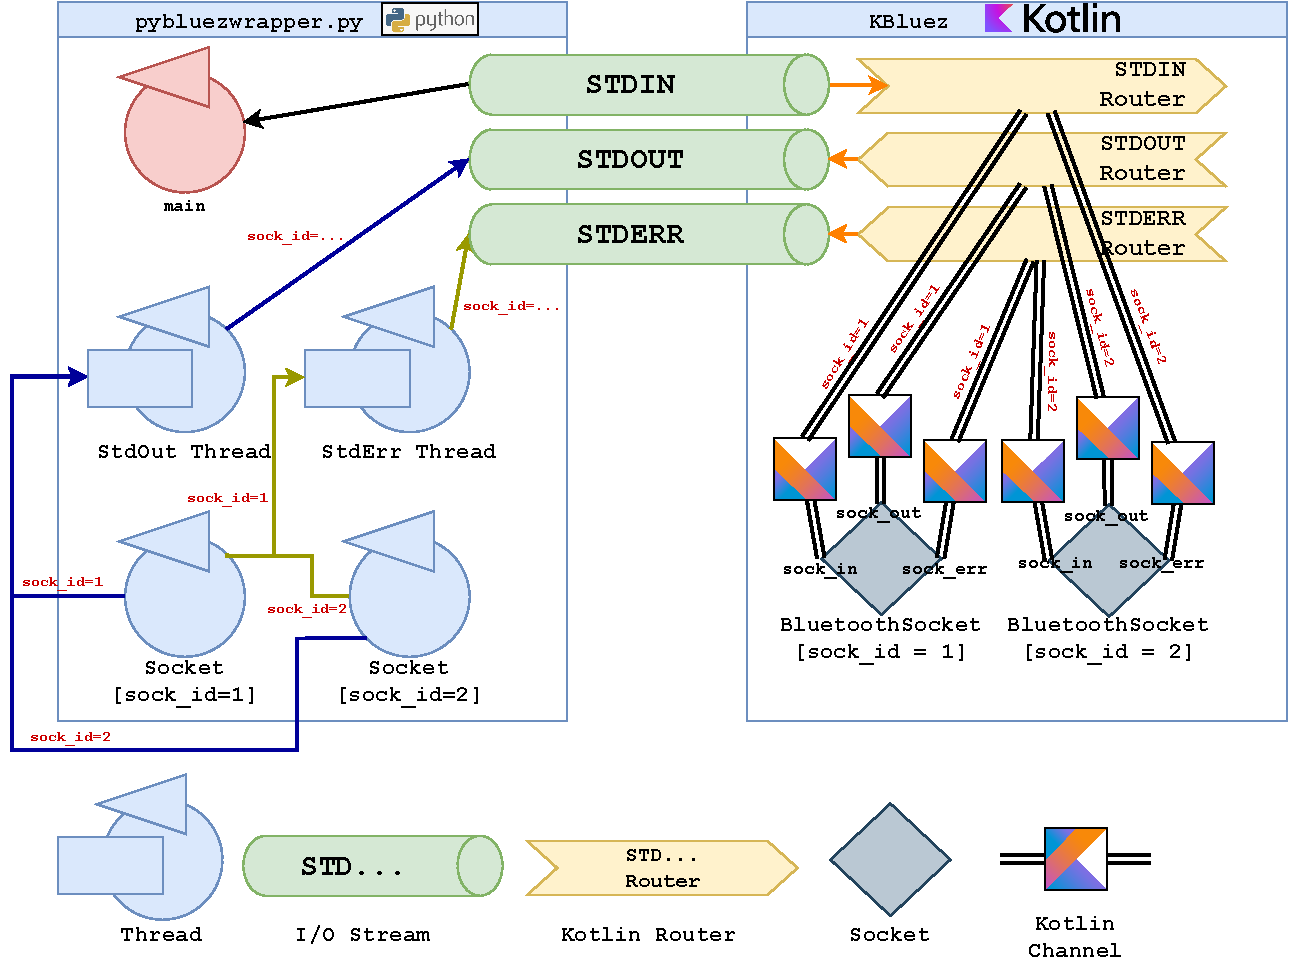
\includegraphics[width=\textwidth]{img/kbluez_general_architecture.pdf}
	\caption{General architecture of the \texttt{KBluez} library}
	\label{fig:kbluez_general_architecture}
\end{figure}

The figure \ref{fig:kbluez_general_architecture} shows a general overview of the architecture of our \texttt{KBluez}.

\begin{figure}[h!]
	\centering
	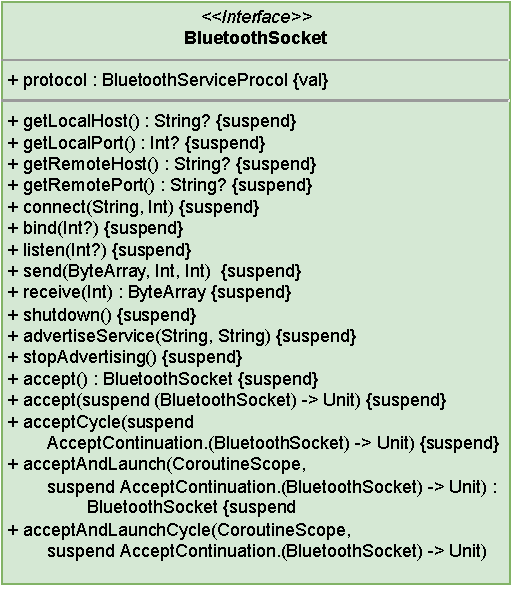
\includegraphics[width=0.4\textwidth]{img/uml_bluetooth_socket_interface.pdf}
	\caption{Class diagram of \texttt{it.unibo.kBluez.socket.BluetoothSocket}}
	\label{fig:uml_bluetooth_socket_interface}
\end{figure}

The figure \ref{fig:uml_bluetooth_socket_interface} shows the class diagram of the \texttt{BluetoothSocket} interface that is the main key point of our library. Other classes will not be shown at the moment.
This interface is implemented by \href{https://github.com/LM-96/MobileSystemProject/blob/main/kBluez/lib/src/main/kotlin/it/unibo/kBluez/pybluez/PyBluezSocket.kt}{PyBluezSocket} class but the implementation will not be exposed in deep.

At the operational point of view, the developer can obtain a \href{https://github.com/LM-96/MobileSystemProject/blob/main/kBluez/lib/src/main/kotlin/it/unibo/kBluez/socket/BluetoothSocket.kt}{\texttt{BluetoothSocket}} with \href{https://en.wikipedia.org/wiki/List_of_Bluetooth_protocols#Radio_frequency_communication_(RFCOMM)}{\texttt{RFCOMM}}by invoking:
\begin{lstlisting}[language=Kotlin]
	val btSock = KBLUEZ.requestNewSocket(BluetoothServiceProtocol.RFCOMM)
\end{lstlisting}
Then, this socket can be used exactly as the internet protocol sockets in order to build a client or a server.

\begin{tcolorbox}
	\begin{center}
		\textbf{We have used \texttt{BluetoothSocket} implementation in order to create a bluetooth server on \texttt{Raspberry} that make it able to communicate with the device of the user. No library or third-party components are needed in \texttt{Android}.}
	\end{center}
\end{tcolorbox}

\subsection{Towards Actor Modeling}

\subsubsection{Running \texttt{QAK} infrastructure under \texttt{Android}}

In the \textit{Mobile System} course we study the fundamentals of \texttt{Android} developing.
We deeply analysed all components offered to the \texttt{Android} developer such as \href{https://developer.android.com/reference/android/app/Activity}{\texttt{Activity}}, \href{https://developer.android.com/guide/components/services}{Services}, \href{https://developer.android.com/reference/android/content/Intent}{\texttt{Intent}},
\href{https://developer.android.com/guide/components/broadcasts}{\texttt{Broadcast Received}}, \href{https://developer.android.com/reference/android/os/AsyncTask}{\texttt{AsyncTask}} and so on and so forth\dots

Now, we want to merge all of these concepts with the already mentioned \texttt{actor meta-modeling} and programming. For these purposes, as anticipated, we have the \texttt{QA-System} that is well documented at the \texttt{Github} \href{https://htmlpreview.github.io/?https://github.com/anatali/issLab2022/blob/main/it.unibo.issLabStart/userDocs/Dispense/lezioni/html/QakIntro.html}{\texttt{repository}} of the corse of \textit{Ingegneria dei Sistemi Software}.

Just to give a fast overview, \textbf{an actor is an active entity that receives messages thanks to a channel that it owns}. So, when an actor receives a message, it performs some action depending on the contents. The \texttt{QAK} system make easy to define and handle actors that are mapped into \texttt{Kotlin} \href{https://developer.android.com/kotlin/coroutines?gclsrc=ds&gclsrc=ds}{coroutines} and, in addition to this, the infrastructure fully supports the concept of \textbf{actors as finite state machine} that change their internal state by receiving messages or \textit{events}.

\textbf{Using actors and \texttt{QAK} let us use \textit{actor meta-modeling} as shown in this \href{https://htmlpreview.github.io/?https://github.com/anatali/issLab2022/blob/main/it.unibo.issLabStart/userDocs/Dispense/lezioni/html/QakIntro.html\#qak-un-esempio-piu-articolato}{example}.}
Once the actor meta-model is well-developed, we can execute it using \texttt{QAK}, but this introduces some problems related with the nature of \texttt{QAK} that works on normal \texttt{JVM}.



\begin{enumerate}
	\item To define an actor, \texttt{QAK} requires it definition in a special \texttt{.pl} file that maintains all the defined actors
	\begin{tcolorbox}
		\begin{center}
			\textbf{We have an extension of the entire \texttt{QAK} infrastructure made by \textit{Luca Marchegiani} at \href{https://github.com/LM-96/QA-Extensions}{\texttt{QA-Extensions} repository} that let the developer use \href{https://kotlinlang.org/docs/annotations.html}{\texttt{Annotations}} instead of \textit{legacy} configuration file.}
		\end{center}
	\end{tcolorbox}

	\item  To define an actor, in addition to annotations or configuration file, the developer must extend \href{https://github.com/LM-96/QA-Extensions/blob/main/it.unibo.qakactor/src/main/kotlin/QActorBasic.kt}{QActorBasic} or \href{https://github.com/LM-96/QA-Extensions/blob/main/it.unibo.qakactor/src/main/kotlin/QActorBasicFsm.kt}{QActorBasicFsm} classes so, since we are using \texttt{Kotlin}, multiple inheritance is not allowed than it is not possible to define classes that extend both \href{https://developer.android.com/reference/android/app/Activity}{\texttt{Activity}} and \texttt{ActorBasicFsm}
	\begin{tcolorbox}
		\begin{center}
			\textbf{We have created a new way to define actors that uses the newest interfaces \href{https://github.com/LM-96/QA-Extensions/blob/android/it.unibo.qakactor/src/main/kotlin/IQActorBasic.kt}{\texttt{IQActorBasic}} and \href{https://github.com/LM-96/QA-Extensions/blob/android/it.unibo.qakactor/src/main/kotlin/IQActorBasicFsm.kt}{\texttt{IQActorBasicFsm}}.}
		\end{center}
	\end{tcolorbox}

	\item \texttt{QAK} creates a log file for each defined actor: this is not easy in \texttt{Android} because of the restrictions for writing files
	\begin{tcolorbox}
		\begin{center}
			\textbf{We have added another modification to the extensions that allows to disable file creation in \href{https://github.com/LM-96/QA-Extensions/blob/android/it.unibo.qakactor/src/main/kotlin/sysUtil.kt}{\texttt{sysUtil}} by adding a simple parameter to the launcher of the \texttt{QA-System} (see \href{https://github.com/LucaLand/MobileSystemsProject-LL/blob/0.9.1/app/src/main/java/it/unibo/mobilesystems/actors/QAKUtils.kt}{QAKUtils.kt}).}
		\end{center}
	\end{tcolorbox}
	
\end{enumerate}

In addition to this, notice that \textbf{\texttt{Android} classes are not compiled in \texttt{.class} but in \texttt{.dex}}, so the annotation scan that is present in the \texttt{QA-Extensions} does not work. To quickly resolve this problem, we choose to declare actor classes in a \textit{hard-coded} way inside the \href{https://github.com/LucaLand/MobileSystemsProject-LL/blob/0.9.1/app/src/main/java/it/unibo/mobilesystems/actors/QAKUtils.kt}{QAKUtils.kt}. Indeed, for extension purposes, the launcher developed in \texttt{QA-Extensions} let the developer to add some parameters, so it is easy to make additional extensions like this.

In future development it is possible to use some more accurate mechanisms such as \href{https://github.com/classgraph/classgraph/wiki/Build-Time-Scanning}{\textit{build time scanning}} of the annotations. 

\subsubsection{\texttt{Coroutines} in \texttt{Android} with \texttt{ViewModel}}

As studied in \textit{Mobile System} course, if an \texttt{Android} developer has to perform a long \texttt{IO} operation inside ad \texttt{Activity}, he should use other components like \href{https://developer.android.com/reference/android/os/AsyncTask}{\texttt{AsyncTask}} that, in simple terms, creates a new thread for the \textit{long-time} operation, and \textit{after} calls a function in which the developer can put the \texttt{UI} updates.

\begin{tcolorbox}[colback=red!5!white,colframe=red!75!black]
	\begin{center}
		\textbf{\texttt{AsyncTask} are now deprecated in favour of the new \texttt{Kotlin} concurrency utilities (see \href{https://developer.android.com/topic/libraries/architecture/coroutines}{\textit{Kotlin} coroutines components} in \texttt{Android}).}
	\end{center}
\end{tcolorbox}

Before we knew this, we had already decided to experiment something new such as \href{https://developer.android.com/topic/libraries/architecture/viewmodel}{\texttt{ViewModel}} that is a component \textit{designed to store and manage UI-related data in a lifecycle conscious way} and that can be used in combination with \texttt{Kotlin} coroutines.

Even without \texttt{ViewModel}, in \texttt{Kotlin} it is easily possible to execute pieces of concurrent code that update \texttt{UI} inside a coroutine. For example, suppose that you have to launch a long \texttt{IO} operation that loads your recipes stored into a database and have to show it on the activity:

\begin{lstlisting}[language=Kotlin]
class BluetoothConnectionActivity : AppCompactActivity() {
	
	lateinit var tableLayout : TableLayout
	val scope : CoroutineScope = ...
	val recipesRepo : RecipesRepo = ...
	
	override fun onCreate(savedInstanceState: Bundle?) {
		tableLayout = findViewById(R.id.recipesTableLayout)
		scope.launch {
			
			//retrieveAll() method uses blocking network IO
			//operations such as read from remote database
			val recipes = recipesRepo.retrieveAll()
			
			withContext(Dispatchers.Main) {
				for(recipe in recipes) {
						//update tableLayout with recipe...
				}
			}
		}
	}
}
\end{lstlisting}

Indeed, the \texttt{launch} primitive \textit{launches} a new coroutine that is dispatched to another thread (or to a pool of threads), but when we called \texttt{Dispatchers.Main} then the block inside is passed to the \textit{main} thread that executes it. So, \textit{UI} updates are performed.

As suggested by \textit{Android} developer guide, instead of this pattern it is better to use \texttt{ViewModel} that automatically manage the lifecycle of the coroutines launched inside this.
We have extended the suggested solution with this pattern:

\begin{lstlisting}[language=Kotlin]
	class RecipesIO(private val recipesRepo : RecipesRepo) {
		
		suspend fun retrieveAll() : Result<List<Recipe>> {
			return withContext(Dispatchers.IO) {
				return@withContext try {
					Result.success(recipesRepo.retrieveAll())
				} catch (e : Exception) {
					Result.failure(e)
				}
			}
		}
				
	}

class RecipesViewModel(private val recipesIO : RecipesIO) {
	
	private val onRetrieved = mutableListOf<
			suspend (Result<List<Recipe>>) -> Unit>()
	
	fun addOnRetrieved(uiUpdate : suspend (Result<List<Recipe>>) -> Unit) {
		onRetrieved.add(uiUpdate)
	}
	
	fun asyncRetrieveAll() {
		viewModelScope.launch{
			val recipes = this@RecipesViewModel.recipesIO.retrieveAll()
			onRetrieved.forEach { uiUpdate ->
				uiUpdate(recipes)
			}
		}
	}
	
}
	
class BluetoothConnectionActivity : AppCompactActivity() {
		
		lateinit var tableLayout : TableLayout
		val recipesRepo : RecipesRepo = ...
		val recipesViewModel = RecipesViewModel(recipesRepo)
		
		override fun onCreate(savedInstanceState: Bundle?) {
			tableLayout = findViewById(R.id.recipesTableLayout)
			recipesViewModel.addOnRetrieved { result ->
					result.onSuccess { recipes ->
						for(recipe in recipes) {
							//update tableLayout with recipe...
						}
					}
					result.onFailure { exception ->
						//Notify failure 
					}
			}
			recipesViewModel.asyncRetrieveAll()
		}
	}
\end{lstlisting}

Notice that \texttt{viewModelScope} is a special \href{https://kotlinlang.org/api/kotlinx.coroutines/kotlinx-coroutines-core/kotlinx.coroutines/-coroutine-scope/}{\texttt{CoroutineScope}} owned by each \texttt{ViewModel} that automatically cancel all coroutines launched inside it if the related owner is cancelled. So, using it is totally safe!

\texttt{Android} let the developer use another special scope that is \href{https://developer.android.com/topic/libraries/architecture/coroutines#lifecyclescope}{\texttt{LifecycleScope}} (see the documentation for details).

This mechanism is very powerful but \textbf{the developer must pay attention and be careful} because if he exaggerates he should saturate the main thread if he forgets to use  \texttt{Dispatcher.IO} for blocking operations.

\subsubsection{From \texttt{Coroutines} to \texttt{QActors}}

We have just shown that an \texttt{Activity} can launch asynchronous operations using coroutines that can also update the \texttt{UI}. So, what could happen if we \textit{transform} an \texttt{Activity} into a \textit{finite state machine actor}?

Indeed, we added some modifications to the \href{https://github.com/LM-96/QA-Extensions}{\texttt{QA-Extensions}} that let the developer define actors \textbf{using an interface} thanks to the \texttt{Kotlin} \href{https://kotlinlang.org/docs/delegated-properties.html}{\textbf{delegates}} that let to make something similar to the multiple inheritance.

\begin{tcolorbox}
	\begin{center}
		\textbf{We create the class \href{https://github.com/LucaLand/MobileSystemsProject-LL/blob/0.9.1/app/src/main/java/it/unibo/mobilesystems/actors/ActorAppCompactActivity.kt}{\texttt{ActorAppCompactActivity}} that automatically \textit{configure} the actor nature of an activity. A class that extends \texttt{ActorAppCompactActivity} is an \texttt{Android} activity that also is a finite state machine actor. The developer must however remember to use the proper \href{https://github.com/LM-96/QA-Extensions/tree/android/it.unibo.qakactor/src/main/kotlin/annotations}{annotations} on his class\footnote{Notice that for instantiation reasons the actors that extends \texttt{ActorAppCompactActivity} \underline{must} be annotated with \texttt{\@StartMode(TransientStartMode.MANUAL)}}.}
	\end{center}
\end{tcolorbox}

\begin{figure}[h!]
	\centering
	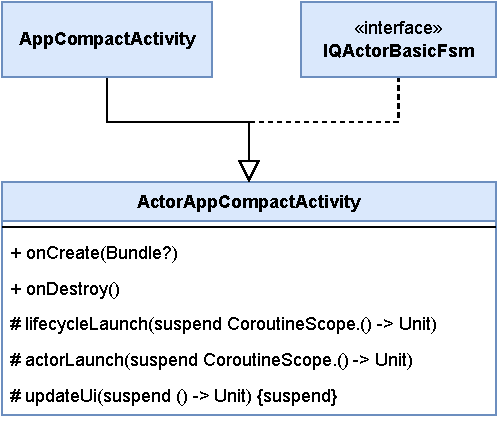
\includegraphics[width=0.5\textwidth]{img/actorappcompactactivity_uml.pdf}
	\caption{Class diagram of \href{https://github.com/LucaLand/MobileSystemsProject-LL/blob/0.9.1/app/src/main/java/it/unibo/mobilesystems/actors/ActorAppCompactActivity.kt}{\texttt{ActorAppCompactActivity}}}
	\label{fig:uml_actorappcompactactivity}
\end{figure}

All the classes that extends \texttt{ActorAppCompactActivity} \underline{\textbf{must}} also use th \texttt{by} keyword offered by \texttt{Kotlin} in order to get the implementation of the \texttt{IQActorBasicClass} following this pattern:
 
\begin{lstlisting}[language=Kotlin]
	val APP_SCOPE = CoroutineScope(SupervisorJob() + Dispatchers.Default)
	val DEFAULT_PARAMS = mutableParameterMap()
	.addBlockIOParam()
	.addAnnotatedClassesParams(
				MyActivity::class.java
	)
	.addSystemScope(APP_SCOPE)

	@QActor("my_ctx")
	@StartMode(TransientStartMode.MANUAL)
	class MyActivity : ActorAppCompactActivity(), IQActorBasicFsm
								by qakActorFsm(MyActivity::class.java,
								Dispatchers.Default,
								DEFAULT_PARAMS)
	{
			...
	}
\end{lstlisting}

If you want to add other activities, you have to add the relative class into \texttt{addAnnotatedClassesParams()} method that builds the \href{https://github.com/LM-96/QA-Extensions/blob/main/it.unibo.qakactor/src/main/kotlin/utils/ParameterUtils.kt}{\texttt{ParameterMap}}. In addition to this, the class must be passed also in the \texttt{qakActorFsm()} method after the \texttt{by} keyword: unlucky, this code repetition is needed because we are in \texttt{Android} so we can use annotation scanning as said.

Notice also the \texttt{APP\_SCOPE}:  this scope is created in order to avoid the use of \href{https://kotlinlang.org/api/kotlinx.coroutines/kotlinx-coroutines-core/kotlinx.coroutines/-global-scope/}{\texttt{GlobalScope}} that is strongly discouraged.

To conclude this overview, we underline these methods:
\begin{itemize}
	\item \underline{\texttt{lifecycleLaunch(block : suspend CoroutineScope.() -> Unit)}}\\
	launches a coroutine that executes the passed \texttt{block} using the \href{https://developer.android.com/reference/kotlin/androidx/lifecycle/LifecycleCoroutineScope}{\texttt{LifecycleCoroutineScope}} associated with the lifecycle of the activity;
	
	\item \underline{\texttt{actorLaunch(block : suspend CoroutineScope.() -> Unit)}}\\
	launches a coroutine that executes the passed \texttt{block} using the \texttt{CoroutineScope} associated with the actor;
	
	\item \underline{\texttt{updateUi(block : suspend () -> Unit)}}\\
	a \texttt{suspend} function that executes the passed \texttt{block} using \href{https://developer.android.com/kotlin/coroutines/coroutines-adv#main-safety}{\texttt{Dispatchers.Main}}; this method can be used from a coroutine in order to perform \texttt{ui} updates.
\end{itemize}

\begin{tcolorbox}
	\begin{center}
		\textbf{In order to prevent the overload of main thread, we decide to use the \href{https://developer.android.com/kotlin/coroutines/coroutines-adv\#main-safety}{\texttt{Dispatchers.Default}} as default dispatcher of all coroutines in which actor are executing, so, if an \textit{activity actor} have to perform \texttt{ui} updates, he can call \texttt{updateUi} method.
			This is the reason why we are using the \texttt{APP\_SCOPE} that is created using \texttt{Dispatchers.Default}.
		}
	\end{center}
\end{tcolorbox}

\subsubsection{Logical architecture}

\begin{figure}[h!]
	\centering
	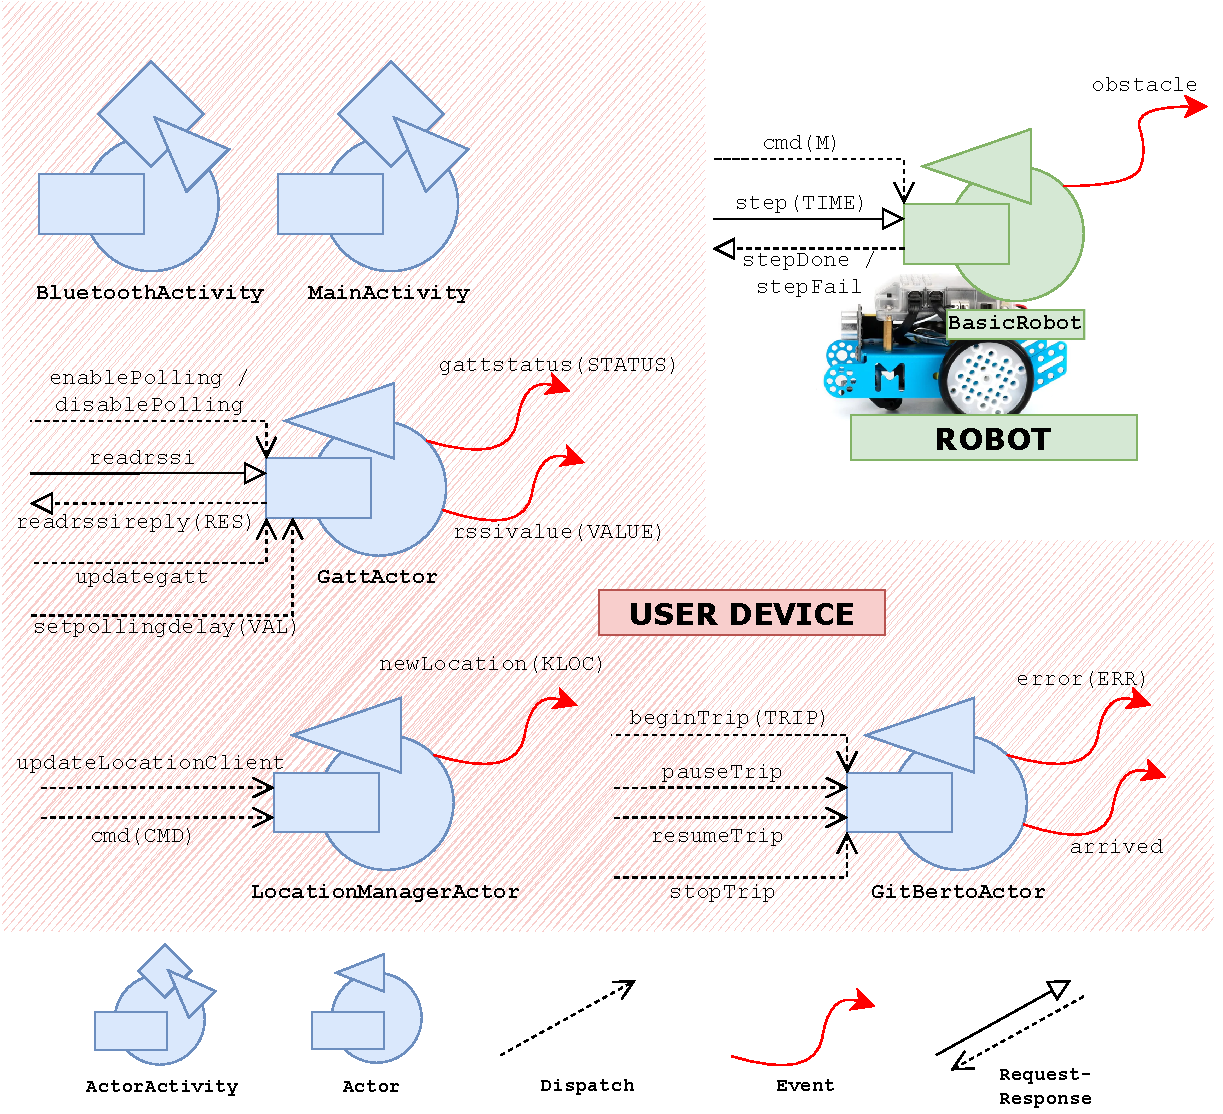
\includegraphics[width=\textwidth]{img/logical_architecture.pdf}
	\caption{Logical architecture of \gitberto system}
	\label{fig:logical_architecture}
\end{figure}

As final result of this very fast analysis, we provide the \textbf{logical architecture} of the \gitberto system in the figure \ref{fig:logical_architecture}.

We can also provide a small description of all the actor that will be present in the \texttt{Android} application of \gitberto system:
\begin{itemize}
	\item \underline{\textbf{BluetoothActivity}}\\
	the activity that makes the user device able to establish a connection with the robot;
	
	 \item \underline{\textbf{MainActivity}}\\
	 the main activity that user can use to set the destination and start the trip;
	 
	 \item \underline{\textbf{GattActor}}\\
	 the actor that uses \texttt{Bluetooth Low Energy} for \href{https://en.wikipedia.org/wiki/Bluetooth_Low_Energy#GATT_operations}{\texttt{GATT}} functionality in order to continuously check the presence of the robot when the connection is established;
	 
	 \item \underline{\textbf{LocationManagerActor}}\\
	 the actor that \textit{manages} the location sending events when user move changing his position;
	 
	 \item \underline{\textbf{LocationManagerActor}}\\
	 the actor that make the system able to interact with the robot using an \textit{high level} view of it; this actor offer the main operations to manage the trip execution.
\end{itemize}
